\documentclass[a4paper, 12pt]{article}
\usepackage[utf8]{inputenc}         %Permite acentuação
\usepackage[brazilian]{babel}       %Adequação para a lingua portugues
\usepackage{courier}                %Pacote fonte de listing que suporta negrito
\usepackage{amsmath}                %Pacote auxiliar para matemática
\usepackage{graphicx}               %Importação de imagem
\usepackage{cite}                   %Pacote de citações
\usepackage{makeidx}                %Pacote para gerar sumário
\usepackage{enumerate}              %Pacote para utilizar o ambiente enumerate
\usepackage{indentfirst}            %Pacote que corrige o espaço dos parágrafos
\usepackage{setspace}               %Pacote de espaçamento entre linhas
\usepackage{enumitem}               %Pacote de ambiente itemize
\usepackage{hyperref}               %Pacote de gerenciamento de hiperlinks
\usepackage{url}                    %Pacote de gerenciamento de urls
\usepackage{siunitx}                %Utilização de unidades do SI
\usepackage{placeins}               %Permite Delimitar até onde uma figura pode aparecer
\usepackage{float}                  %Especificar onde a figura deve ficar
\usepackage{listings}               %Pacote que permite adicionar códigos ao texto
\usepackage{amssymb}                %Pacote de símbolos matemáticos
\usepackage{graphics,graphicx}      %Adicionar caixas de texto
\usepackage{fancybox}               %Pacote para a inserção de caixas de texto
\usepackage{booktabs}               %Pacote para adicionar tabelas lado a lado
\usepackage{subfig}                 %pacote para criação de subfiguras

%Margem padrão ABNT
\usepackage[left=3.00cm, right=2.00cm, top=3.00cm, bottom=2.00cm]{geometry}                                         
%Configuração das cores para link
\hypersetup{
    colorlinks=true,       % false: boxed links; true: colored links
    linkcolor=black,          % color of internal links (change box color with linkbordercolor)
    citecolor=black,        % color of links to bibliography
    filecolor=black,      % color of file links
    urlcolor=blue           % color of external links
    }
    
%Define language for AMPL
\lstdefinelanguage{AMPL}{keywords={set,param,var,arc,integer,minimize,maximize,subject,to,node,sum,in,Current,complements,integer,solve_result_num,IN,contains,less,suffix,INOUT,default,logical,sum,Infinity,dimen,max,symbolic,Initial,div,min,table,LOCAL,else,option,then,OUT,environ,setof ,union,all,exists,shell_exitcodeuntil,binary,forall,solve_exitcodewhile ,by,if,solve_messagewithin,check,in,solve_result
},sensitive=true,comment=[l]{\#}}

\lstset{%
    language = AMPL,
    breaklines = true,
    frame = lrtb,
    basicstyle = \footnotesize\ttfamily,
    commentstyle=\textit,
    tabsize = 1,
   % keywordstyle=\bfseries,
    extendedchars=true,
    literate={á}{{\'a}}1 {ã}{{\~a}}1 {é}{{\'e}}1 {ç}{{\c{c}}}1 {ó}{{\'o}}1 {ê}{{\^e}}1 {â}{{\^a}}1 {ô}{{\^o}}1 {í}{{\'i}}1 {õ}{{\~o}}1
}
            %Arquivo de configuração do projeto

\begin{document}
    \onehalfspacing                         %Ajusta espaço entre linhas para 1.5
    %======================= PRIMEIRA FOLHA INTERNA  ============================%
\begin{titlepage}
\begin{figure}[H]
    \begin{minipage}{.5\linewidth}
        \flushleft
        
\includegraphics[width=.94in, height=1in,
            keepaspectratio=true]{01_img/logo_unicamp.jpg}
    \end{minipage}%
    \begin{minipage}{.5\linewidth}
        \flushright
        
\includegraphics[width=.94in, height=1in,
            keepaspectratio=true]{01_img/logo_feec.png}
    \end{minipage} 
\end{figure}

    
    \begin{center}
    \large{Universidade Estadual de Campinas}\\
    \large{Faculdade de Engenharia Elétrica e de Computação}
    \end{center}
    
    
    \vspace*{4.8cm}
    
    \begin{center}
    {\sc \Large  Reconfiguração das redes de distribuição de energia elétrica operando em diferentes níveis de demanda}
    \end{center}
    
    
    \vspace*{3.25cm}
    \begin{minipage}{7cm}
    \small
    
    \rule{6.9cm}{0.2mm} \hfill 
    \end{minipage}
    
    Aluno/Bolsista: Lucas Zenichi Terada
    
    \vspace*{1.25cm}
    \begin{minipage}{7cm}
    \small
    
    \rule{6.9cm}{0.2mm} \hfill 
    \end{minipage}

    Orientador: Prof. Dr. Marcos Julio Rider Flores
    
    
    \null \vfill
    
    \begin{center}
    Campinas\\2018
    \end{center}
\end{titlepage}
%============================= FOLHA DE ROSTO ================================%


\begin{center}
\large Universidade Estadual de Campinas\\
Faculdade de Engenharia Elétrica e de Computação
\end{center}

\vspace*{1.0cm}
\begin{center}
\large Lucas Zenichi Terada
\end{center}

    
\vspace*{1.3cm}
    
\begin{center}
    {\sc Reconfiguração das redes de distribuição de energia elétrica operando em diferentes níveis de demanda}
\end{center}
    
\vspace*{0.5cm}

    
\vspace*{1.0cm}
    
\begin{flushright}
\begin{minipage}{11.0cm}
Projeto de iniciação científica financiada pela Fundação de Amparo e Pesquisa do Estado de São Paulo. Realizado na Faculdade de Engenharia Elétrica e de Computação da UNICAMP no nível de graduação.
    
\vspace*{0.5cm}
    
\vspace*{1.0cm}
Orientador: Marcos Julio Rider Flores
    
\end{minipage}
\end{flushright}
    
\null \vfill
\begin{minipage}{7cm}
\small
Este exemplar corresponde ao relatório parcial do projeto de iniciação científica.    
\rule{6.9cm}{0.2mm} \hfill 
\end{minipage}
    
\null \vfill
\begin{center}
    Campinas\\2018
\end{center}
\thispagestyle{empty}
\newpage         %Adiciona a página de capa do projeto
    {\large\textbf{Resumo das atividades}}      %Resumo de atividades do bolsista

{\large\textbf{Resumo}}                     %Resumo do projeto

\clearpage                                  %Quebra de página

\listoffigures                              %Adiciona a lista de figuras

\clearpage                                  %Quebra de página

\listoftables                               %Adiciona a lista de tabelaas

\clearpage                                  %Quebra de página






\clearpage                                  %Quebra de página             %Adiciona página de elementos pré textuais
    \tableofcontents                        %Adiciona o sumário no documento
    \section{Introdução}

Os sistemas de distribuição de energia elétrica (SDEE) são planejados como redes de malhas interconectadas. Com a finalidade de operar de forma mais eficiente de modo a coordenar a proteção do sistema mais facilmente e reduzir a corrente de curto circuito, o SDEE opera com uma topologia radial \cite{Romais2014ReconfiguracaoMista}.

Os SDEE devem operar de forma a respeitar tanto as restrições de carga quanto as restrições operacionais. Dado que o sistema está operando em regime permanente é interessante operá-lo em estado de mínimas perdas. Para isso reconfigura-se o sistema de distribuição de modo a reduzir as perdas ôhmicas ao longo da rede.

O problema de reconfiguração do sistema de distribuição (RSD) é um problema de planejamento da operação das chaves alocadas ao longo dos alimentadores e consiste na abertura e/ou fechamento das chaves com o objetivo de melhorar um índice de desempenho.

A reconfiguração ótima é uma importante ferramenta para aumentar a confiabilidade de um SDEE, especialmente quando a automação avançada e tecnologias de redes inteligentes (smartgrids) tornam-se mais importantes e mais acessíveis às concessionarias de distribuição.

Os benefícios ao reduzir as perdas de potência ativa no sistema de distribuição são:% : -> são:
             % ao -> de se
\begin{itemize}
    \item Alívio do sistema de distribuição: com a redução das perdas de potência ativa, o sistema é aliviado, o que leva a uma maior vida útil dos equipamentos, uma maior capacidade de fornecimento e um melhor perfil da magnitude de tensão no sistema;
   % a um -> um (você não colocou esse a antes do segundo item, "uma maior capacidade", mas colocou antes desse terceiro. Acho que não está errado, só estranhei)---Feito
    \item Adiamento de investimentos para a expansão do sistema de distribuição: a redução das perdas de potência tem como consequência a redução dos fluxos de potência nos condutores, e desta forma é adiada a necessidade de reforços na rede.
    
    \item Melhoria na qualidade de energia: a reconfiguração melhora o perfil da magnitude de tensão do sistema;
    
    % não seria "adiamento"?
    \item Adiamento da necessidade de ampliação da capacidade de transmissão: a rede de distribuição pode reduzir o carregamento de linhas de transmissão no horário de pico, aumentando efetivamente a capacidade de transmissão;
    
    \item Adiamento da ampliação da capacidade de geração: menos unidades de geração operando são necessárias no horário de pico;
    
    \item Redução do uso de combustíveis: ao reduzir as perdas, reduz-se a necessidade de geração de energia a partir de fontes não renováveis, o que leva a uma economia no uso de combustíveis fósseis;
    
    \item Benefícios ambientais: a redução no uso de combustíveis fósseis tem como consequência a redução de poluição;
    
    \item Redução na contratação de energia elétrica para grandes clientes: ao reduzir as perdas das redes dos grandes clientes, reduz-se o consumo de energia elétrica.
\end{itemize}

A reconfiguração do sistema de distribuição é um problema de otimização cuja modelagem matemática pode ser classificada das seguintes formas, como descrito em \cite{Goncalves2013ModelosRadiais}:

\begin{itemize}
    \item PL: Programação Linear
    
    \item PNL: Programação não linear
    
    \item PLIM: Programação linear inteiro misto
    
    \item PNLIM: Programação não linear inteiro misto
\end{itemize}

Para solucionar esses problemas utilizam-se de ``solvers'' que são programas cuja finalidade é encontrar uma solução ótima para um problema de programação.

Problemas de PL podem ser resolvidos usando algoritmos convencionais como simplex e pontos interiores.
Já para problemas de PNL existem diversas técnicas como método de Newton e relaxação Lagrangeana.
Problemas de PLIM podem ser resolvidos usando técnicas baseadas em branch and bound.
Por fim um problema de PNLIM são complicados de serem solucionados e imagina-se que solvers comerciais usem algoritmos baseados em \emph{branch and bound}. % comerciais usam -> comerciais usem (não tenho certeza...) -- Feito
%talvez o uso de um termo em inglês como "branch and bound" fique melhor se escrito em itálico (mesma coisa pra sentença anterior)
O problema de RSD, como será visto, é um problema não linear inteiro misto.
Problemas não lineares são complicados de serem solucionados devido à dificuldade de convergência dos algoritmos usados para determinar soluções ótimas. %devido a -> devido à (só pensar em reestruturar a frase para "por causa da dificuldade de...". Como a frase ficou com um "da" ao invés de um "de" (troque por um "de" e veja como fica estranho) antes da palavra dificuldade, então existe um artigo "a" antes de "dificuldade". Como "devido" tem a preposição "a", então você acaba com dois "a", virando um "à". Espero ter mais exclarecido do que confundido :D)
Além disso, em problemas de PL e PLIM existem condições necessárias e suficientes de otimização teoricamente provadas que garantem se uma dada solução é factível ou não.
Já para problemas PNL e PNLIM não existem tais condições. Por outro lado existem as heurísticas e meta-heurísticas que buscam resolver esses problemas de forma a buscar uma solução satisfatória em tempo adequado \cite{Goncalves2013ModelosRadiais}.  

%Trabalho realizados anteriormente
% redes radias -> redes radiais
Alguns trabalhos relevantes na literatura que abordam a reconfiguração de redes radiais com demandas fixas foram tratados em \cite{Baran1989NetworkBalancing } abordando algoritmos heurísticos%faltou um ponto final

Algoritmos genéticos como mostrado em  \cite{Souza2015AlgoritmoVariaveis} se mostraram interessantes para resolver problemas de característica não linear.
Em \cite{deCastro2002AnOptimization} mostra-se uma interessante abordagem que simula o comportamento do sistema imunológico do corpo humano para solucionar um problema de otimização não linear.
Outra abordagem interessante é a transformação de um problema PNLIM em um problema PCSOIM (programação cônica de segunda ordem inteiro misto) através do relaxamento de uma restrição do problema \cite{Romais2014ReconfiguracaoMista}.            %Adiciona a introdução do documento
    \section{Objetivos}

Com a finalidade de reduzir as perdas ôhmicas ao longo da rede, esse projeto tem o objetivo de propor uma nova topologia que atenda os requisitos de um SDEE. Para isso ele deve propor uma nova topologia que, obrigatoriamente, deve ser uma topologia radial e deve obedecer as limitações de operação da mesma.              %Adciona a seção de objetivos
    \section{Metodologia}

O modelo para reconfiguração do sistema de distribuição de energia elétrica, abordado nesse projeto, foi implementado na linguagem de de modelagem matemática (AMPL).

\subsection{Introdução a Linguagem de Programação Matemática}

O AMPL é uma linguagem de modelagem algébrica cuja função é descrever e resolver problemas a partir do seu modelo matemático. 
A linguagem fora desenvolvida nos ``Bells Labs'' por Robert Fourer, David Gay e Brian Kernighan com o intuito de ajudar as pessoas a comunicar modelos de otimização para sistema de computação, aproveitando o poder e a conveniência de formulações algébricas familiares \cite{ampl}. 
Possui, atualmente, suporte para uma grande diversidade de ``solvers'' tanto comerciais quanto códigos abertos .

\subsection{``Solvers'' comerciais}

Os ``solvers'' usados no AMPL, como dito anteriormente, podem ser tanto comerciais quanto constituídos de código aberto.
Ambos as categorias podem resolver determinados problemas de acordo com a natureza do sistema. 

\subsection{Hipóteses e definições da formulação do problema}

\begin{figure}[H]
    \centering
    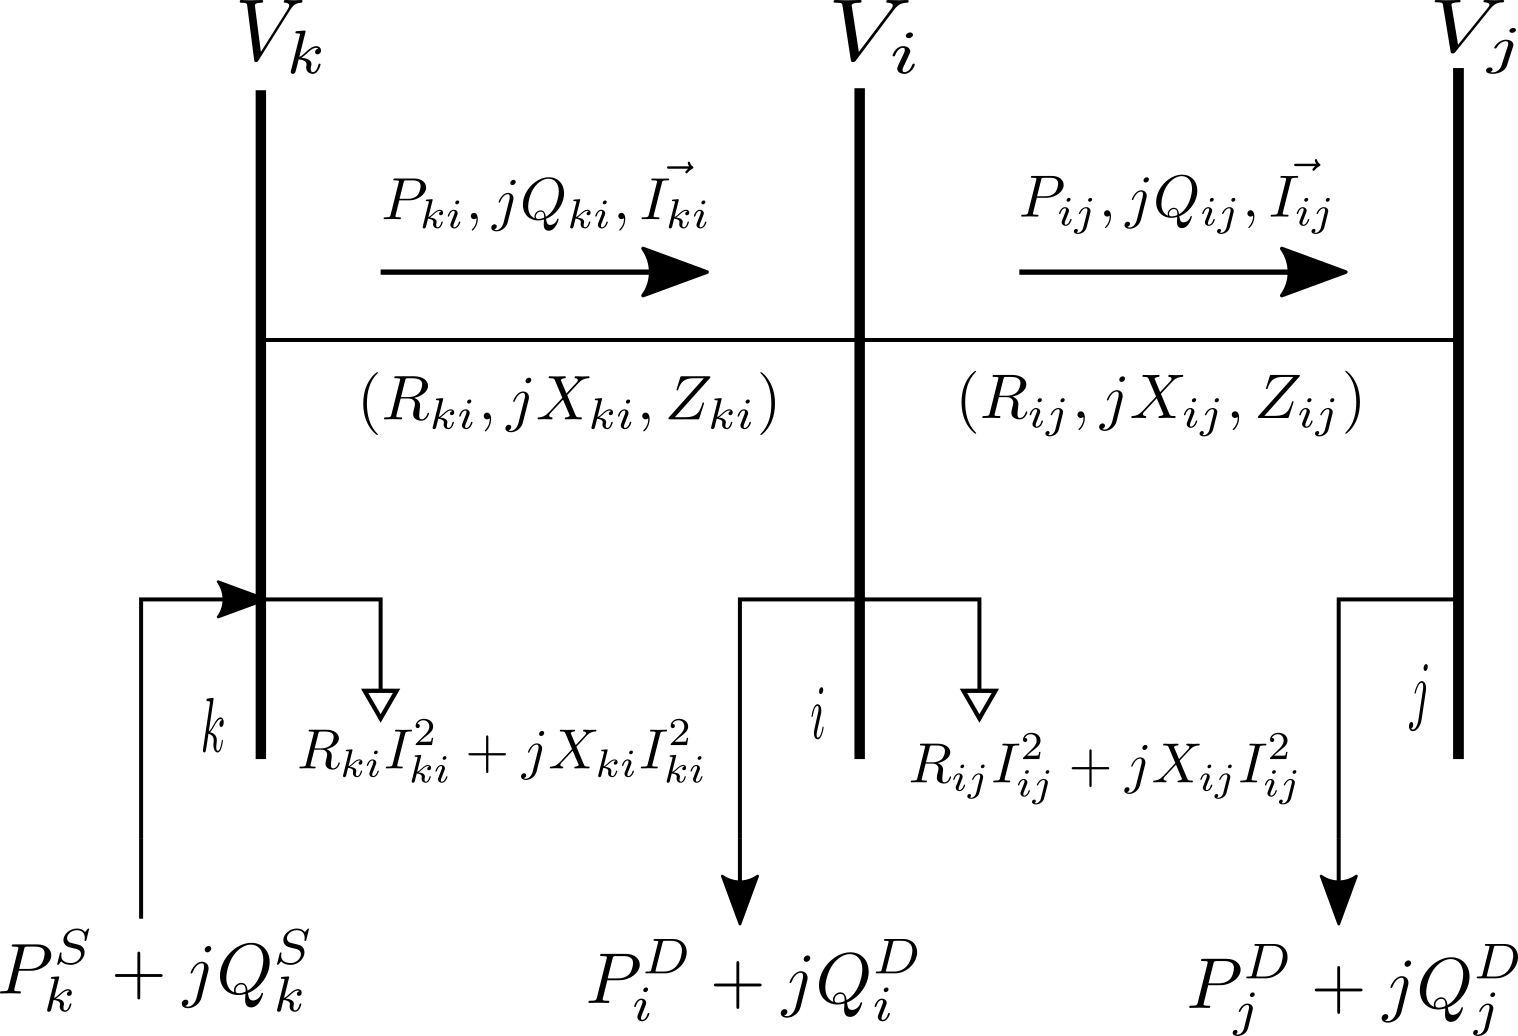
\includegraphics[scale = 1.2]{01_img/diagrama_nos.png}
    \caption{Sistema de distribuição radial}
    \label{fig:SDR}

\end{figure}

Hipóteses adotadas:
Visando representar o funcionamento em regime permanente de um sistema de distribuição de energia, são feitas as seguintes hipóteses (comumente usadas nas formulações de varredura de fluxo de carga \textbf{citar Shirmohammadi1988ANetworks} e mostradas na figura \ref{fig:SDR}.

\begin{itemize}
    \item As demandas nas cargas na rede de distribuição são representadas como potência ativa e reativas contantes;
    
    \item O sistema é balanceado e representado pelo seu equivalente monofásico;
    
    \item As perdas de potência ativa e reativa no circuito \textit{ij} estão concentradas no nó \textit{i}.
    
    \item As chaves são representadas como circuito curtos de impedância nula.
\end{itemize}

\subsection{Modelo de otimização}

O modelo de otimização interpretado pelo AMPL possui a seguinte forma:

{\raggedleft
\shadowbox{
\begin{minipage}{\dimexpr\textwidth-\shadowsize-2\fboxrule-2\fboxsep-8pt}
    
    \begin{center}
        Minimizar: Função objetivo        
    \end{center}

\hspace{2cm}Sujeito a:

    \begin{center}
        Restrições físicas\\
        Restrições operativas\\
    \end{center}
\end{minipage}
}}

As restrições do problema devem ser tais que modelem as leis da física que regem um sistema de distribuição de energia elétrica e as faixas com as quais essas grandezas podem operar ao longo da rede.
Para isso define-se dois conjuntos de restrições, restrições físicas e restrições operativas.

             %Adciona seção de metodologia
    \section{Modelagem do problema}

\subsection{Função objetivo}

Dado o modelo de otimização a ser interpretado pelo AMPL, é possível definir a função objetivo com base na figura~\ref{fig:SDR}.
A fim de reduzir as perdas ôhmicas na rede elétrica, a função objetivo do problema consiste em minimizar a somatória das perdas por resistência elétrica no conjunto de circuitos do sistema.

Definindo $c^{lss}$ como parâmetro que representa o custo das perdas de potência ativa na rede têm-se:

\begin{equation}
    \text{Min} = c^{lss}\sum_{ij\in\Omega_{l}}R_{ij}I_{ij}^{2}
\end{equation}

Tal que, $\Omega_{l}$ é o conjunto de circuitos do sistema.
            %Adiciona seção de restrições
    \subsection{Balanço de potência}

\begin{figure}[H]
    \centering
    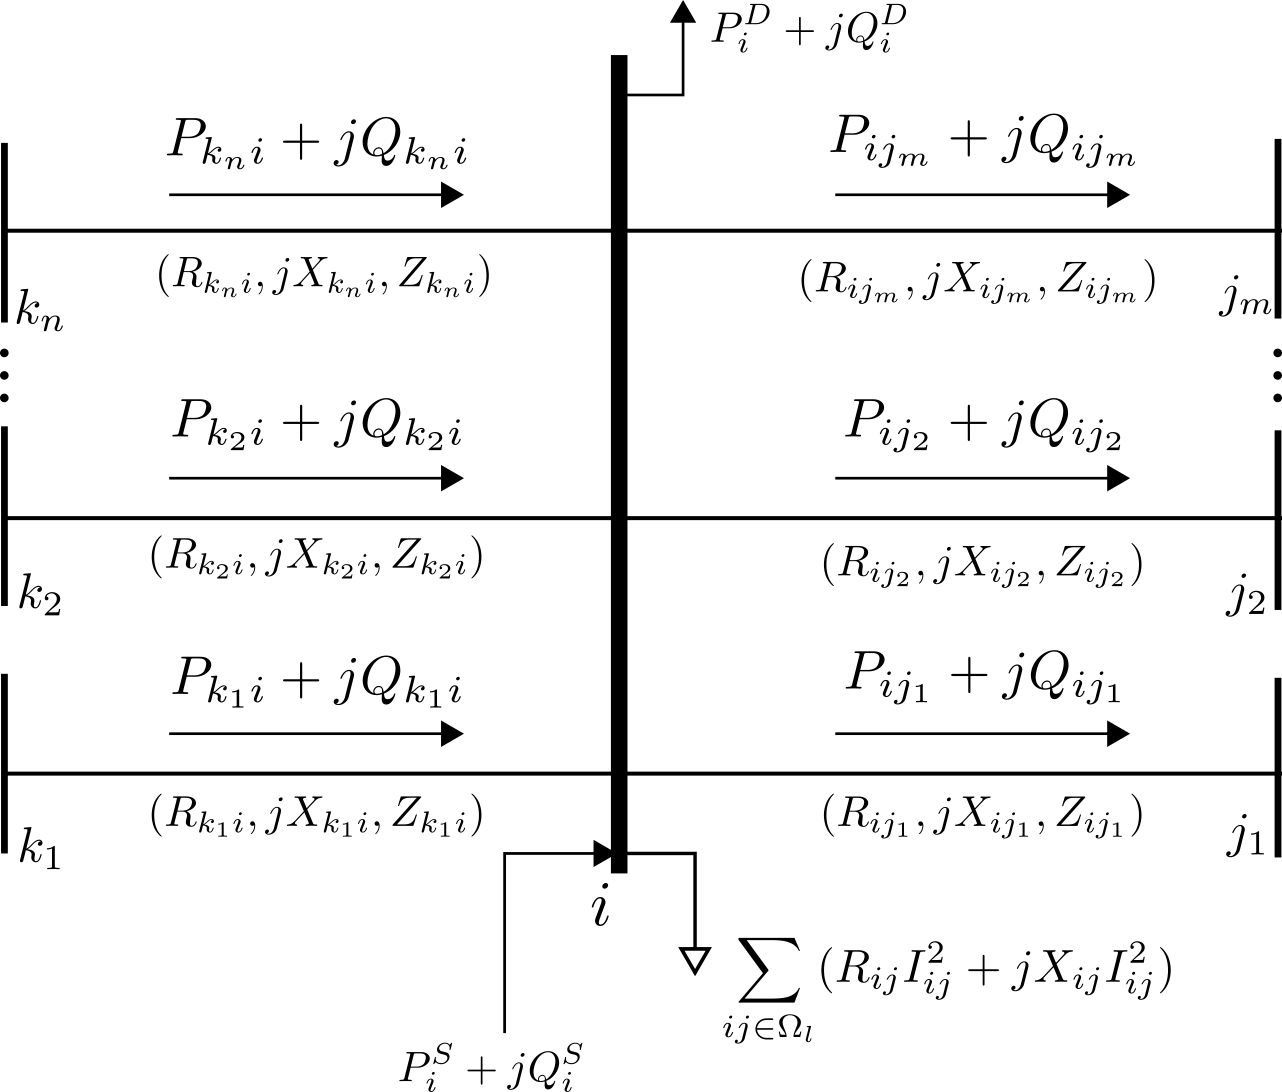
\includegraphics[scale = 1.4]{01_img/diagrama_potencia.png}
    \caption{Exemplo de um diagrama de balanço de potência entre nós de um sistema de distribuição de energia elétrica}
    \label{fig:balanco_pot}
\end{figure}

A figura~\ref{fig:balanco_pot} representa a forma expandida da figura~\ref{fig:SDR}, para melhor compreensão do problema de balanço de potência, onde $m$ e $n$ representam um número qualquer de nós ligados ao nó $i$. 
Para isso considere que nos parâmetros e variáveis que representam um ramo, o primeiro subíndice representa o nó de partida e o segundo subíndice o nó de chegada (exemplo: $P_{12}$ representa o fluxo de potência ativa que vai do nó 1 para o nó 2).

Seja $P_{i}^{D}$ e $Q_{i}^{D}$ potência ativa e reativa demandada no nó i respectivamente e $P_{i}^{S}$ e $Q_{i}^{S}$ potência ativa e reativa gerada no nó i respectivamente, têm-se que:

\begin{equation*}
    \sum_{ki\in\Omega_{l}}P_{ki} - \sum_{ij\in\Omega_{l}}(P_{ij} + R_{ij}I_{ij}^{2}) + P_{i}^{S} = P_{i}^{D}\quad\forall i \in\Omega_{b}
\end{equation*}

\begin{equation*}
    \sum_{ki\in\Omega_{l}}Q_{ki} - \sum_{ij\in\Omega_{l}}(Q_{ij} + X_{ij}I_{ij}^{2}) + Q_{i}^{S} = Q_{i}^{D}\quad\forall i \in\Omega_{b}
\end{equation*}

Dado que $\Omega_{b}$ é o conjunto de nós do sistema.
É possível mudar a variável \textit{k} pela variável \textit{j}, uma vez que ambas pertencem ao conjunto $\Omega_{l}$ e os somatórios envolvendo-as estão desconectadas, desse modo:

\begin{equation}
    \sum_{ji\in\Omega_{l}}P_{ji} - \sum_{ij\in\Omega_{l}}(P_{ij} + R_{ij}I_{ij}^{2}) + P_{i}^{S} = P_{i}^{D}\quad\forall i \in\Omega_{b}\label{eq:fluxo_pot_ativa}  
\end{equation}


\begin{equation}
    \sum_{ji\in\Omega_{l}}Q_{ji} - \sum_{ij\in\Omega_{l}}(Q_{ij} + X_{ij}I_{ij}^{2}) + Q_{i}^{S} = P_{i}^{D}\quad\forall i \in\Omega_{b}\label{eq:fluxo_pot_reativa}
\end{equation}

O sistema de equações não lineares em \ref{eq:fluxo_pot_ativa} e \ref{eq:fluxo_pot_reativa} representam a operação em regime permanente de uma rede elétrica radial e são frequentemente utilizados no método de varredura de fluxo de carga \cite{Shirmohammadi1988ANetworks} e \cite{Cespedes1990NewNetworks}               %Adiciona seção de restrição
    \subsection{Queda de tensão entre nós}


Formulação do Problema de Fluxo de Carga para redes elétricas radiais:

Da figura \ref{fig:SDR}, a queda de tensão do circuito é definida pela equação \ref{eq:queda_tensao}.

\begin{equation}
    \Vec{V}_{i} - \Vec{V}_{j} = I_{ij}(R_{ij} + jX_{ij})\quad\forall ij \in \Omega_{l}
    \label{eq:queda_tensao}
\end{equation}

Em que $\Omega_{l}$ é o conjunto de circuitos. %OBSERVAÇÃO: Explicar mais sobre o conjunto de circuitos
Através da fórmula para o cálculo da potência aparente, $I_{ij}$ pode ser calculado usando a equação \ref{eq:corrente_ramo}.

\begin{equation}
    I_{ij} = \left(\frac{P_{ij} + jQ_{ij}}{\Vec{Vj}}\right)^{*}\quad\forall ij \in \Omega_{l}
    \label{eq:corrente_ramo}
\end{equation}

%OBSERVAÇÃO: Explicar o uso da tensão Vj e as potências (Considerou-se que as perdas ao longo do ramo ij estão concentradas no nó i, por isso a potência que passa ao longo do ramo é a potência Sij que é igual a potência drenada do nó j

Substituindo $I_{}ij$ da equação \ref{eq:corrente_ramo} na equação \ref{eq:queda_tensao} obtém-se a equação \ref{eq:queda_tensao_pot} que define a queda de tensão em função das potências e impedâncias do circuito.

Seja $(P_{ij} + jQ_{ij})^{*} = (P_{ij} - jQ_{ij})$ logo:

\begin{equation}
    (\Vec{V}_{i} - \Vec{V}_{j})\Vec{V}_{j}^{*} = (P_{ij} - jQ_{ij})(R_{ij} + jX_{ij}) \quad\forall ij \in \Omega_{l}
    \label{eq:queda_tensao_pot}
\end{equation}

Considerando que $\Vec{V}_{i} = V_{i}\angle{\theta_{i}}$, $\Vec{V}_{j} = V_{j}\angle{\theta_{j}}$ e $\theta_{ij} = \theta_{i} - \theta_{j}$, tal que  $V_{i}$ e $V_{j}$ representam as magnitudes da tensão em seus respectivos nós bem como $\theta_{i}$ e $\theta_{j}$ representam seus ângulos.
Dessa forma a equação \ref{eq:queda_tensao_pot} pode ser escrita decompondo a fase de suas exponenciais, como mostra a equação \ref{eq:queda_tensao_sencos}.

\begin{equation}\label{eq:queda_tensao_sencos}
    V_{i}V_{j}[cos\theta_{ij} + jsen\theta_{ij}] - V_{j}^{2} = (P_{ij} - jQ_{ij})(R_{ij} + jX_{ij}) \quad\forall ij \in \Omega_{l}
\end{equation}

Identificando as partes real e imaginária na equação \ref{eq:queda_tensao_sencos}, obtém-se:

\begin{equation}
    V_{i}V_{j}cos\theta_{ij} = V_{j}^{2} + (R_{ij}P_{ij} + X_{ij}Q_{ij})\quad\forall ij \in \Omega_{l}
    \label{eq:queda_tensao_real}
\end{equation}

\begin{equation}
    V_{i}V_{j}sen\theta_{ij} = X_{ij}P_{ij} - R_{ij}Q_{ij}\quad\forall ij \in \Omega_{l}
    \label{eq:queda_tensao_imaginaria}
\end{equation}

Usando a fórmula da trigonometria, que é a relação básica entre o seno e o cosseno, $sen^{2}(\theta_{ij}) + cos^{2}(\theta_{ij}) = 1$, e somando os quadrados das equações \ref{eq:queda_tensao_real} e \ref{eq:queda_tensao_imaginaria}, obtém-se:

\begin{equation}
    V_{i}^{2} - 2(R_{ij}P_{ij} + X_{ij}Q_{ij}) - Z_{ij}^{2}I_{ij}^{2} - V_{j}^{2} = 0\quad\forall ij \in \Omega_{l}
    \label{eq:queda_tensao_restricao}
\end{equation}

Note que a equação \ref{eq:queda_tensao_restricao} não depende da diferença angular entre as tensões, e é possível obter a magnitude da tensão do nó ($V_j$) em termos da magnitude inicial ($V_i$), o fluxo de potência ativa ($P_{ij}$), o fluxo de potência reativa ($Q_{ij}$), a magnitude do fluxo de corrente ($I_{ij}$) e os parâmetros elétricos do ramo \textit{ij}.


             %Adiciona seção de restrição
    \subsection{Fluxo de corrente em um ramo}

Na equação de queda de tensão, a magnitude do fluxo de corrente $I_{ij}$ é mostrado na equação \ref{eq:corrente_magnitude} calculado a partir do produto com seu complexo conjugado.

\begin{equation}
    I_{ij}^{2} = \frac{P_{ij}^{2}+Q_{ij}^{2}}{V_{j}^{2}}\quad\forall ij \in \Omega_{l}
    \label{eq:corrente_magnitude}
\end{equation}
             %Adiciona seção de restrição
    \subsection{Restrições operativas do sistema}

Como visto as equações \ref{eq:fluxo_pot_ativa}, \ref{eq:fluxo_pot_reativa}, \ref{eq:queda_tensao_restricao} e \ref{eq:corrente_magnitude}
são restrições cujas variáveis $V_{i}$ e $I_{ij}$ estão sempre na forma quadrática, por isso é possível fazer uma substituição de variável a fim de tornar mais simples o problema, tal que:

\begin{align*}
    I_{ij}^{sqr} = I_{ij}^{2} \text{ e } V_{i}^{sqr} = V_{i}^{2} 
\end{align*}

Dessa forma é possível determinar as restrições operativas para o funcionamento da SDEE.

\subsubsection{Limites de tensão}

Em um sistema de distribuição de energia elétrica é preciso garantir que a tensão em um nó deva estar dentro de uma faixa de operação determinada por norma, por isso uma restrição fundamental para o problema é a restrição de limites de tensão em um nó, determinada pela seguinte equação:

\begin{equation}
    \underline{V}^{2} \leq V_{i}^{sqr} \leq \overline{V}^{2}\qquad i \in\Omega_{b}
\end{equation}

Onde $\underline{V}$ e $\overline{V}$ representam os limites inferiores e superiores de tensão, respectivamente, que uma rede pode possuir.



\subsubsection{Limite de corrente}

Assim como as tensões, o fluxo de corrente também deve ser limitado para não comprometer o SDEE.
Assim a equação que descreve a restrição é:

\begin{equation}
    0 \leq I_{ij}^{sqr} \leq \overline{I}_{ij}^{2} \qquad ij\in\Omega_{l} 
\end{equation}

\subsubsection{Chaves presentes no sistema}

Para reconfiguração do SDEE, existem chaves ao longo da rede que podem ser modificadas de modo a garantir a operação desejada.
Considere as seguintes restrições:

\begin{figure}[h]
    \centering
    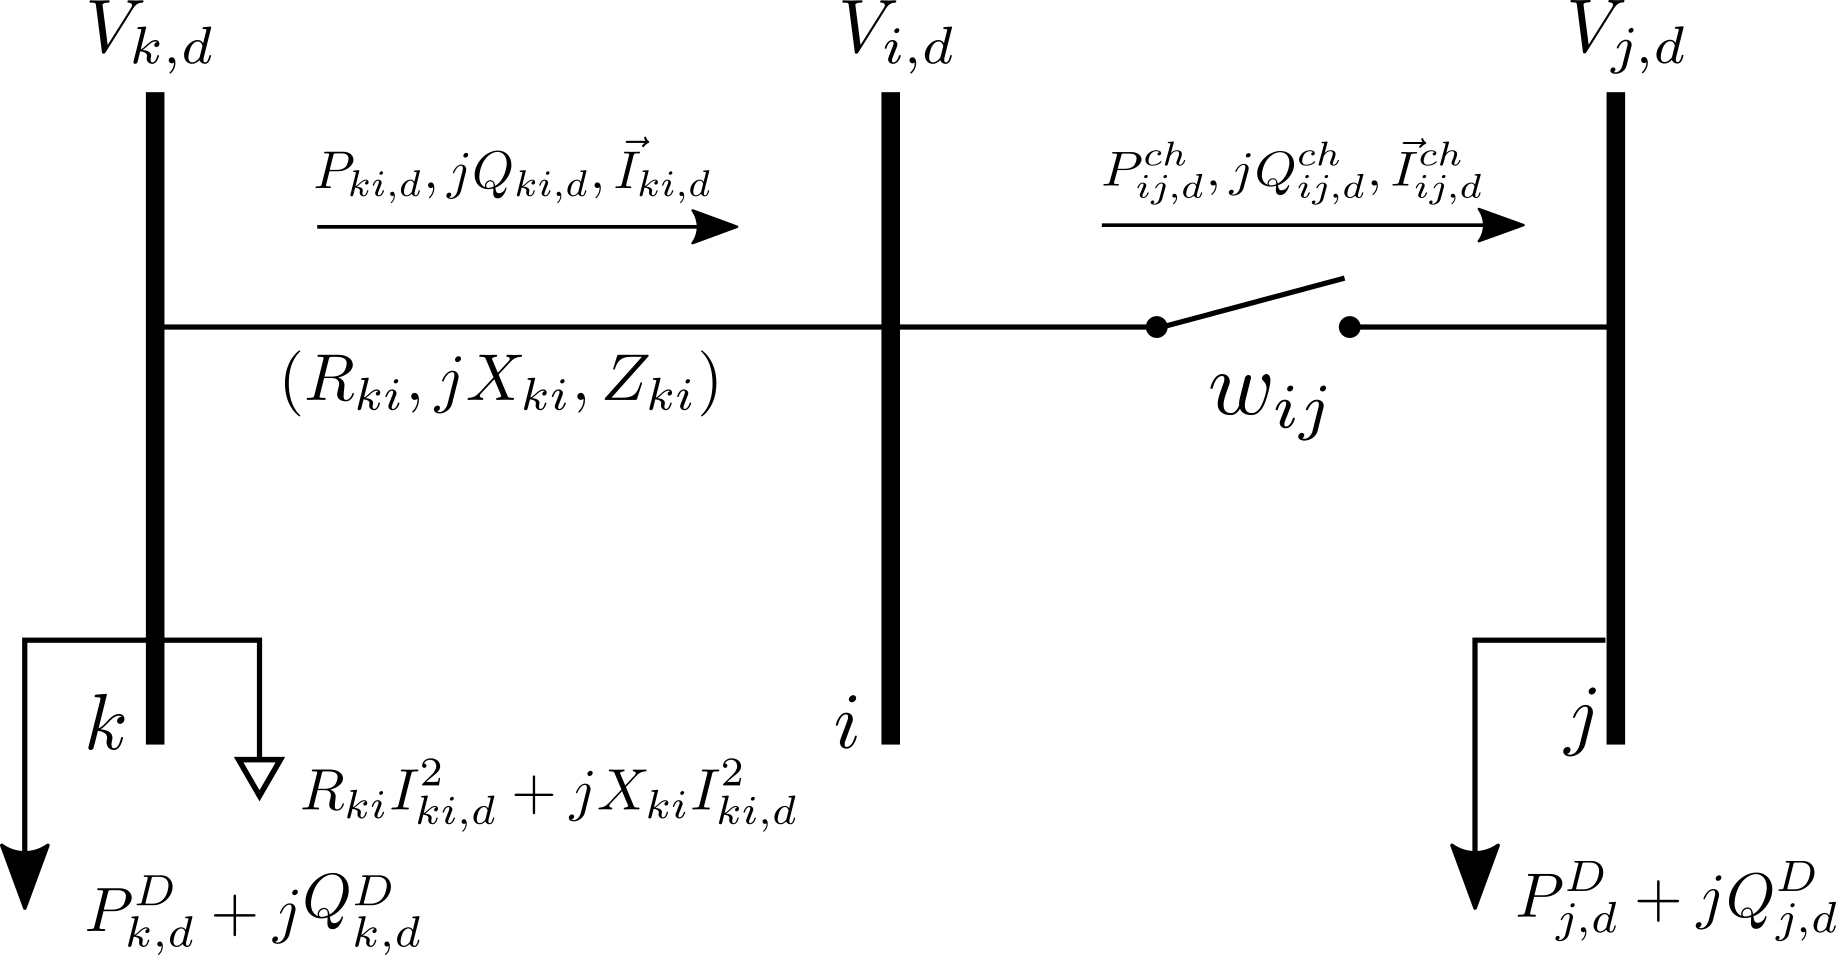
\includegraphics[scale = 1.5]{01_img/diagrama_chaves.png}
    \caption{Modelo de uma Cl conectada entre dois nós}
    \label{fig:diagrama_chave}
\end{figure}
    
\begin{itemize}
    \item Balanço de potência
\end{itemize}
    Com base na figura \ref{fig:diagrama_chave} faz-se necessário reformular as equações de balanço de potência adicionando as variáveis que representam as chaves na modelagem do problema.
    
\begin{equation}
    \sum_{ji\in\Omega_{l}}P_{ji} - \sum_{ij\in\Omega_{l}}(P_{ij} + R_{ij}I_{ij}^{sqr})+ \sum_{ji\in\Omega_{ch}}P_{ji}^{ch} -\sum_{ij\in\Omega_{ch}}P_{ij}^{ch} + P_{i}^{S} = P_{i}^{D}\quad\forall i \in\Omega_{b}\label{eq:fluxo_pot_ativa_chaves}  
\end{equation}
    
    
\begin{equation}
    \sum_{ji\in\Omega_{l}}Q_{ji} - \sum_{ij\in\Omega_{l}}(Q_{ij} + X_{ij}I_{ij}^{sqr})+ \sum_{ji\in\Omega_{ch}}Q_{ji}^{ch} -\sum_{ij\in\Omega_{ch}}Q_{ij}^{ch} + Q_{i}^{S} = P_{i}^{D}\quad\forall i \in\Omega_{b}
    \label{eq:fluxo_pot_reativa_chaves}
\end{equation}
    
Onde $\Omega_{ch}$ representa o conjunto de chaves da rede elétrica e $w_{ij}$ é uma variável binária que representa o estado da chave \textit{ij}, se $w_{ij} = 1$ a chave ij está fechada, caso contrário a chave está aberta, ver figura~\ref{fig:diagrama_chave}. $P_{ij}^{ch}$ e $Q_{ij}^{ch}$ representam o fluxo de potência ativa e reativa da chave \textit{ij}.
    
As restrições expressas nas equações \ref{eq:fluxo_pot_ativa_chaves} e \ref{eq:fluxo_pot_reativa_chaves} são uma extensão das equações \ref{eq:fluxo_pot_ativa} e \ref{eq:fluxo_pot_reativa}, considerando a presença de chaves na rede elétrica.
    
Além do balanço de potência outras restrições devem ser estabelecidas devido a presença de chaves, são elas:
    
\begin{itemize}
    \item Diferença de tensões entre dois nós conectadas por uma chave
\end{itemize}

    
A diferença de tensão entre nós, na presença de chaves, deve ser igual a zero, uma vez que, de acordo com as hipóteses adotadas, a impedância da chaves é representada como uma impedância nula.
Sendo assim, usando as variável binária $w_{ij}$ é possível equacionar a restrição da seguinte forma:
    
\begin{equation}
    -(\overline{V}^{2} - \underline{V}^{2})(1-w_{ij}) \leq V_{i}^{sqr} - V_{j}^{sqr} \leq (\overline{V}^{2} - \underline{V}^{2})(1-w_{ij})\qquad ij\in\Omega_{ch}        
\end{equation}
    
Note que se $w_{ij}$ for igual a 1 (chave fechada), a diferença entre as tensões no nó $i$ e nó $j$ será igual a zero, o que condiz a hipótese adotada.
\begin{itemize}
   \item Fluxo de potência na chave
\end{itemize} 
    
O fluxo de potência na chave é determinada pelas equações abaixo.
    
\begin{equation}
    -(\overline{V}\,\overline{I}_{ij}^{ch})w_{ij} \leq P_{ij}^{ch} \leq (\overline{V}\,\overline{I}_{ij}^{ch})w_{ij}\qquad ij\in\Omega_{ch}   
\end{equation}
    
    
\begin{equation}
    -(\overline{V}\,\overline{I}_{ij}^{ch})w_{ij} \leq Q_{ij}^{ch} \leq (\overline{V}\,\overline{I}_{ij}^{ch})w_{ij}\qquad ij\in\Omega_{ch}   
\end{equation}
    
Note que se a variável $w_{ij}$ for igual a 0 (chave aberta) o fluxo de potência na chave é igual a zero o que condiz com a proposta do elemento de circuito na rede, quando igual a 1 as restrições representam o fluxo máximo de potência ativa e reativa permitida na chave quando está energizada.

\subsubsection{Restrição de radialidade}

A representação de um SDEE é feita através de nós e circuitos. Fazendo analogia com a teoria de grafos, um SDEE pode ser considerado como um grafo formado por n arcos e m nós.
Da teoria de grafos, uma árvore é um grafo conexo sem ciclos, assim é possível comparar a topologia radial de um SDEE com uma árvore.
Como mostrado em \cite{Bazaraa1990LinearFlows}, a árvore de um grafo é um sub-grafo com ($m-1$) arcos.

Assim, pode-se dizer que a topologia de um SDEE com $n_{b}$ nós é radial se satisfaz as duas seguintes condições: Condição 1: a solução deve apresentar ($n_{b}$) circuitos; e Condição 2: a solução deve gerar uma topologia conexa. Note que a restrição de radialidade tem que ser formada pelas condições 1 e 2.
Somente a condição 1 não garante a radialidade do SDEE. O problema de RSD cumpre com as seguintes características: 1) apenas uma única subestação existente no SDEE (nó da subestação); 2) todos os outros nós são nós de carga; 3) a primeira lei de kirchhoff, deve ser cumprida, e 4) o objetivo é encontrar a melhor topologia radial. 
A condição 1 é satisfeita pela seguinte restrição:

\begin{equation}
    |\Omega_{l}| + \sum_{ij\in\Omega_{ch}}w_{ij} = |\Omega_{b}| - 1
    \label{eq:radialidade}
\end{equation}

Em que $|\Omega|$ é um operador que calcula o número de elementos do conjunto $\Omega$.

Uma solução que satisfaz a restrição de balanço de potência (primeira Lei de Kirchhoff) tem de fornecer a demanda de potência em cada nó de carga. De modo que existe um caminho entre a subestação e os nós de carga. Portanto, cada nó está ligado com a subestação, formando um grafo conexo, o que comprova a Condição 2. 
Assim, quando as restrições de balanço de potência são combinadas com a Condição 1, cada nó de carga está ligada por um único caminho com a subestação, isto é, o SDEE é conexo, sem malhas.

\begin{figure}[H]
    \centering
    
\includegraphics[scale = 1]{01_img/restricao_fail.png}
    \caption{Exemplo de rede não radial que obedece a equação \ref{eq:radialidade}}
    \label{fig:radialidade_wrong}
\end{figure}

Observe que a figura \ref{fig:radialidade_wrong}, embora respeite a equação \ref{eq:radialidade} (5 ramos para 6 nós), não é uma topologia radial. Isso pode acontecer se levar somente em consideração a equação \ref{eq:radialidade}.

\begin{figure}[H]
    \centering
    
\includegraphics[scale=0.8]{01_img/restricao_radialidade.png}
    \caption{Exemplo de rede radial que obedece a equação \ref{eq:radialidade}}
    \label{fig:radialidade_right}
\end{figure}

Observe agora a figura \ref{fig:radialidade_right}, note que ela é uma topologia radial, como dito anteriormente é necessário duas condições para garantir tal configuração, como no problema já existem equações que garantem a primeira Lei de Kirchhoff, a topologia final será radial. 
Observe que todos os nós estão interligados, direto ou indiretamente, com o nó 1 (nó da subestação). 
Isso acontece pois as equações de balanço de potência obrigam que haja fluxo de potência para atender as demandas dos mesmos.

Assim a equação \ref{eq:radialidade} junto com \ref{eq:fluxo_pot_ativa_chaves} e \ref{eq:fluxo_pot_reativa_chaves} fornecem as condições necessárias para e suficientes para garantir uma topologia final radial \cite{Lavorato2012ImposingProblems}.

           %Adiciona seção de restrição
    \section{Modelo matemático do problema}
\subsection{Modelagem do problema}


Com base nas deduções e hipóteses adotadas anteriormente, o problema de reconfiguração de uma rede elétrica radial pode ser representado utilizando um modelo de programação linear inteiro misto (PNLIM), mostrado a seguir:

\begin{equation*}
    \text{Min} = c^{lss}\sum_{ij\in\Omega_{l}}R_{ij}I_{ij}^{sqr}
\end{equation*}

Sujeito a:

\begin{equation*}
    \sum_{ji\in\Omega_{l}}P_{ji} - \sum_{ij\in\Omega_{l}}(P_{ij} + R_{ij}I_{ij}^{sqr})+ \sum_{ji\in\Omega_{ch}}P_{ji}^{ch} -\sum_{ij\in\Omega_{ch}}P_{ij}^{ch} + P_{i}^{S} = P_{i}^{D}\quad\forall i \in\Omega_{b}  
\end{equation*}
    
\begin{equation*}
    \sum_{ji\in\Omega_{l}}Q_{ji} - \sum_{ij\in\Omega_{l}}(Q_{ij} + X_{ij}I_{ij}^{sqr})+ \sum_{ji\in\Omega_{ch}}Q_{ji}^{ch} -\sum_{ij\in\Omega_{ch}}Q_{ij}^{ch} + Q_{i}^{S} = Q_{i}^{D}\quad\forall i \in\Omega_{b}
\end{equation*}

\begin{equation*}
    V_{i}^{sqr} - 2(R_{ij}P_{ij} + X_{ij}Q_{ij}) - Z_{ij}^{2}I_{ij}^{sqr} - V_{j}^{sqr} = 0\quad\forall ij \in \Omega_{l}
\end{equation*}

\begin{equation*}
    V_{j}^{sqr}I_{ij}^{sqr} = P_{ij}^{2}+Q_{ij}^{2}\quad\forall ij \in \Omega_{l}
\end{equation*}

\begin{equation*}
    -(\overline{V}^{2} - \underline{V}^{2})(1-w_{ij}) \leq V_{i}^{sqr} - V_{j}^{sqr} \leq (\overline{V}^{2} - \underline{V}^{2})(1-w_{ij})\qquad ij\in\Omega_{ch}        
\end{equation*}
    
\begin{equation*}
    -(\overline{V}\,\overline{I}_{ij}^{ch})w_{ij} \leq P_{ij}^{ch} \leq (\overline{V}\,\overline{I}_{ij}^{ch})w_{ij}\qquad ij\in\Omega_{ch}
\end{equation*}
    
    
\begin{equation*}
    -(\overline{V}\,\overline{I}_{ij}^{ch})w_{ij} \leq Q_{ij}^{ch} \leq (\overline{V}\,\overline{I}_{ij}^{ch})w_{ij}\qquad ij\in\Omega_{ch}   
\end{equation*}
    
\begin{equation*}
    |\Omega_{l}| + \sum_{ij\in\Omega_{ch}}w_{ij} = |\Omega_{b}| - 1
\end{equation*}

\begin{equation*}
    \underline{V}^{2} \leq V_{i}^{sqr} \leq \overline{V}^{2}\qquad i \in\Omega_{b}
\end{equation*}

\begin{equation*}
    0 \leq I_{ij}^{sqr} \leq \overline{I}_{ij}^{2} \qquad ij\in\Omega_{l} 
\end{equation*}

\begin{equation*}
    w_{ij}\quad\text{binário}\qquad\forall ij \in\Omega_{ch}
\end{equation*}

\subsection{Não linearidade}

A não linearidade desse problema está relacionada a restrição expressa na equação~\ref{eq:corrente_magnitude} a qual envolve o produto de duas variáveis quadráticas do sistema, bem como a presença de variáveis binárias ($w_{ij}$), caracterizando-se como um problema de programação não linear inteiro misto.
Dessa forma o problema não pode ser resolvido por \emph{solvers} lineares tais como CEPLEX e sim por programas capazes de resolve-lo como o Knitro e Bonmin, por exemplo.

             %Adiciona a formulação do problema
    \section{Implementando o PNLIM}

A implementação do problema de programação não linear inteiro misto, obtido da análise física e operativa da rede, no AMPL é dada a partir de 3 arquivos principais.
O arquivo de extensão .mod possui a modelagem do problema com base na formulação algébrica das restrições adequado a linguagem do AMPL. 

\lstinputlisting[language=AMPL,caption=Arquivo que contém o programa que modelo o problema de reconfiguração de sistema de distribuição radial, label={lst:mod_file}]{02_code/PNLIM_RSD.mod}

Os demais arquivos principais de extensão \verb|.dat| e \verb|.run| estão nos anexos, juntamente com arquivos auxiliares.


%\gls{}
                 %Adiciona o programa de otimização
    \section{Resultados}
\subsection{Simulação da rede de 45 nós}

Para computar os resultados, utilizou o programa mostrado anteriormente contido no arquivo \verb|PNLIM.mod| presente na listagem~\ref{lst:mod_file}, o qual contem a modelagem do problema de RSD. 
Nos aquivos \verb|PNLIM.dat| e \verb|Sistema45nos.dat| estão contidos os arquivos de dados (com pontos iniciais já definidos) e os parâmetros da rede, respectivamente mostrados nas listagens~\ref{lst:dat_file} e \ref{lst:sist45nos}.

Por fim fora executado o arquivo \verb|PNLIM.run|, presente na listagem~\ref{lst:run_file}, com o auxílio do arquivo \verb|impressao.inc|, na listagem~\ref{lst:imp}. O arquivo de extensão \verb|.run| possui a chamada do modelo, dados e solver responsável pela execução, o arquivo de extensão \verb|.inc| possui comandos para a impressão de dados na tela.

Para encontrar a solução ótima utilizou o \emph{solver} comercial Knitro.


\begin{table}[H]
    \label{tab:impedancia}
    \caption{Parâmetros de impedância e corrente máxima para o conjunto de circuitos da rede didática de 45 nós}
    \begin{minipage}{.5\linewidth}
        \centering
        \begin{tabular}{|c|c|c|c|c|}
        \hline
        $b_\text{part}$ & $b_\text{cheg}$& R [$\Omega$]  & X [$\Omega$] & Imax [A]\\ \hline
         2 &  3 & 0.0922 & 0.0470 & 200\\ \hline
         3 &  4 & 0.4930 & 0.2511 & 200\\ \hline
         4 &  5 & 0.3660 & 0.1864 & 200\\ \hline
         5 &  6 & 0.3811 & 0.1941 & 200\\ \hline
         6 &  7 & 0.8190 & 0.7070 & 200\\ \hline
         7 &  8 & 0.1872 & 0.6188 & 200\\ \hline
         9 & 10 & 0.7114 & 0.2351 & 200\\ \hline
        10 & 11 & 10.300 & 0.7400 & 200\\ \hline
        11 & 13 & 10.440 & 0.7400 & 200\\ \hline
        13 & 14 & 0.1966 & 0.0650 & 200\\ \hline
        14 & 15 & 0.3744 & 0.1238 & 200\\ \hline
        15 & 16 & 14.680 & 11.550 & 200\\ \hline
        17 & 18 & 0.5416 & 0.7129 & 200\\ \hline
        18 & 19 & 0.5910 & 0.5260 & 200\\ \hline
        19 & 20 & 0.7463 & 0.5450 & 200\\ \hline
        20 & 21 & 12.890 & 17.210 & 200\\ \hline
        21 & 22 & 0.7320 & 0.5740 & 200\\ \hline
         3 & 23 & 0.1640 & 0.1565 & 200\\ \hline        
        \end{tabular}
        
    \end{minipage}%
    \begin{minipage}{.5\linewidth}
        \centering
        \begin{tabular}{|c|c|c|c|c|}
        \hline
        $b_\text{part}$ & $b_\text{cheg}$& R [$\Omega$]  & X [$\Omega$] & Imax [A]\\ \hline    
        24 & 25 & 15.042 & 13.554 & 200\\ \hline
        25 & 26 & 0.4095 & 0.4784 & 200\\ \hline
        26 & 27 & 0.7089 & 0.9373 & 200\\ \hline
         4 & 30 & 0.4512 & 0.3083 & 200\\ \hline
        31 & 32 & 0.8980 & 0.7091 & 200\\ \hline
        32 & 33 & 0.8960 & 0.7011 & 200\\ \hline
         7 & 35 & 0.2030 & 0.1034 & 200\\ \hline
        36 & 37 & 0.2842 & 0.1447 & 200\\ \hline
        37 & 38 & 10.590 & 0.9337 & 200\\ \hline
        38 & 39 & 0.8042 & 0.7006 & 200\\ \hline
        39 & 40 & 0.5075 & 0.2585 & 200\\ \hline
        41 & 42 & 0.9744 & 0.9630 & 200\\ \hline
        42 & 43 & 0.3105 & 0.3619 & 200\\ \hline
        43 & 44 & 0.3410 & 0.5302 & 200\\ \hline
        10 & 28 & 20.000 & 20.000 & 200\\ \hline
        12 & 19 & 20.000 & 20.000 & 200\\ \hline
        18 & 29 & 20.000 & 20.000 & 200\\ \hline
        22 & 45 & 0.5000 & 0.5000 & 200\\ \hline
        34 & 39 & 0.5000 & 0.5000 & 200\\ \hline
        \end{tabular}
    \end{minipage} 
\end{table}

\begin{table}[H]
    \label{tab:demanda}
    \caption{Potência ativa e reativa de demanda para cada nó da rede didática de 45 nós}
    
    \begin{minipage}{.5\linewidth}
        \centering

        \begin{tabular}{|c|c|c|c|}
            \hline
            $\Omega_b$ & $T_b$ & $P_D$ [kW] & $Q_D$ [kVar]\\ \hline
            1  &  1 &  0.001 &  0.001\\ \hline 
            2  &  0 &  0.001 &  0.001\\ \hline
            3  &  0 &   30.0 &   10.0\\ \hline
            4  &  0 &   30.0 &   10.0\\ \hline
            5  &  0 &   40.0 &   15.0\\ \hline
            6  &  0 &   20.0 &   10.0\\ \hline
            7  &  0 &   20.0 &    5.0\\ \hline
            8  &  0 &   60.0 &   30.0\\ \hline
            9  &  0 &  0.001 &  0.001\\ \hline
            10 &  0 &   60.0 &   30.0\\ \hline
            11 &  0 &   20.0 &    5.0\\ \hline
            12 &  0 &  0.001 &  0.001\\ \hline
            13 &  0 &   20.0 &    5.0\\ \hline
            14 &  0 &   15.0 &   10.0\\ \hline
            15 &  0 &   20.0 &   10.0\\ \hline
            16 &  0 &  0.001 &  0.001\\ \hline
            17 &  0 &   20.0 &   10.0\\ \hline
            18 &  0 &   40.0 &   15.0\\ \hline
            19 &  0 &   20.0 &    5.0\\ \hline
            20 &  0 &   20.0 &    5.0\\ \hline
            21 &  0 &   20.0 &    5.0\\ \hline
            22 &  0 &   30.0 &   10.0\\ \hline
            23 &  0 &  0.001 &  0.001\\ \hline
                 
        \end{tabular}
        
    \end{minipage}%
    \begin{minipage}{.5\linewidth}
        \centering
         \begin{tabular}{|c|c|c|c|} 
            \hline
            $\Omega_b$ & $T_b$ & $P_D$ [kW] & $Q_D$ [kVar]\\ \hline
            24 &  0 &   30.0 &   10.0\\ \hline
            25 &  0 &   30.0 &   10.0\\ \hline
            26 &  0 &   30.0 &   10.0\\ \hline
            27 &  0 &   30.0 &   10.0\\ \hline
            28 &  0 &  0.001 &  0.001\\ \hline
            29 &  0 &  0.001 &  0.001\\ \hline
            30 &  0 &   30.0 &   10.0\\ \hline
            31 &  0 &  0.001 &  0.001\\ \hline
            32 &  0 &  140.0 &   60.0\\ \hline
            33 &  0 &  140.0 &   60.0\\ \hline
            34 &  0 &  0.001 &  0.001\\ \hline
            35 &  0 &   20.0 &    5.0\\ \hline
            36 &  0 &  0.001 &  0.001\\ \hline
            37 &  0 &   20.0 &    5.0\\ \hline
            38 &  0 &   20.0 &    5.0\\ \hline
            39 &  0 &   40.0 &   15.0\\ \hline
            40 &  0 &   60.0 &   30.0\\ \hline
            41 &  0 &  0.001 &  0.001\\ \hline
            42 &  0 &   50.0 &   10.0\\ \hline
            43 &  0 &   70.0 &   30.0\\ \hline
            44 &  0 &   20.0 &    5.0\\ \hline
            45 &  0 &  0.001 &  0.001\\ \hline

            
            \end{tabular}
    \end{minipage} 
\end{table}


\begin{table}[H]
    \centering
    \caption{Estado das chaves antes da otimização}
    \label{tab:est_chave_atual}
    \begin{tabular}{|c|c|c|c|}
        \hline
        \multicolumn{2}{|c|}{$\Omega_{ch}$} & $w_{ij}$ & $I_{maxch}$ [A]\\ \hline
         1 &   2 &  1 &   500\\ \hline
         8 &   9 &  1 &   500\\ \hline
        11 &  12 &  0 &   500\\ \hline
        16 &  17 &  1 &   500\\ \hline
        23 &  24 &  1 &   500\\ \hline
        26 &  28 &  0 &   500\\ \hline
        27 &  29 &  0 &   500\\ \hline
        30 &  31 &  1 &   500\\ \hline
        33 &  34 &  0 &   500\\ \hline
        35 &  36 &  1 &   500\\ \hline
        40 &  41 &  1 &   500\\ \hline
        44 &  45 &  0 &   500\\ \hline
    \end{tabular}
\end{table}

%Identificar o perfil de tensão ao longo da rede de distribuição


\begin{figure}[H]
    \centering
    
\includegraphics[width=\textwidth]{01_img/rede_inicial.png}
    \caption{Estado inicial da rede de distribuição com alimentador no nó 1}  
    \label{fig:rede_inic}
\end{figure}

\begin{table}[H]\footnotesize
    \caption{Fluxo de potência reativa entre nós no sistema de 45 nós atual}
    \label{tab:fluxo_kW_atual}
    \begin{minipage}{.5\linewidth}
        \centering
        \begin{tabular}{|c|c|c|}
            \hline
            \multicolumn{2}{|c|}{$\Omega_l$} & $P_{ij}$ [kW]  \\ \hline
             2 &   3 & 1293.97\\ \hline
             3 &   4 & 1131.21\\ \hline
             4 &   5 &  785.09\\ \hline
             5 &   6 &  741.52\\ \hline
             6 &   7 &  714.26\\ \hline
             7 &   8 &  377.37\\ \hline
             9 &  10 &  316.12\\ \hline
            10 &  11 &  244.39\\ \hline
            11 &  13 &  214.30\\ \hline
            13 &  14 &  194.15\\ \hline
            14 &  15 &  178.89\\ \hline
            15 &  16 &  151.18\\ \hline
            17 &  18 &  130.97\\ \hline
            18 &  19 &   90.86\\ \hline
            19 &  20 &   70.78\\ \hline
            20 &  21 &   50.02\\ \hline
            21 &  22 &   30.00\\ \hline
             3 &  23 &  122.09\\ \hline
        \end{tabular}
    \end{minipage}%
    \begin{minipage}{.5\linewidth}
        \centering
        \begin{tabular}{|c|c|c|}
            \hline
            \multicolumn{2}{|c|}{$\Omega_l$} & $P_{ij}$ [kW]  \\ 
            \hline
            24 &  25 &   90.04\\ \hline
            25 &  26 &   60.01\\ \hline
            26 &  27 &   30.00\\ \hline
             4 &  30 &  311.55\\ \hline
            31 &  32 &  280.31\\ \hline
            32 &  33 &  140.00\\ \hline
             7 &  35 &  316.06\\ \hline
            36 &  37 &  295.63\\ \hline
            37 &  38 &  261.72\\ \hline
            38 &  39 &  240.82\\ \hline
            39 &  40 &  200.42\\ \hline
            41 &  42 &  140.05\\ \hline
            42 &  43 &   90.00\\ \hline
            43 &  44 &   20.00\\ \hline
            10 &  28 &    0.00\\ \hline
            12 &  19 &   -0.00\\ \hline
            18 &  29 &    0.00\\ \hline
            22 &  45 &    0.00\\ \hline
            34 &  39 &   -0.00\\ \hline        
        \end{tabular}
    \end{minipage} 
\end{table}


  



\begin{table}[H]\footnotesize
    \caption{Fluxo de potência reativa entre nós no sistema de 45 nós atual}
    \label{tab:fluxo_kvar_atual}
    \begin{minipage}{.5\linewidth}
        \centering
        \begin{tabular}{|c|c|c|}
            \hline
            \multicolumn{2}{|c|}{$\Omega_l$} & $Q_{ij}$ [kVar]  \\ \hline
             2  &  3 &  498.36\\ \hline
             3  &  4 &  441.02\\ \hline
             4  &  5 &  297.33\\ \hline
             5  &  6 &  280.51\\ \hline
             6  &  7 &  264.25\\ \hline
             7  &  8 &  149.64\\ \hline
             9  & 10 &  119.23\\ \hline
            10  & 11 &   88.38\\ \hline
            11  & 13 &   82.67\\ \hline
            13  & 14 &   77.62\\ \hline
            14  & 15 &   67.53\\ \hline
            15  & 16 &   51.47\\ \hline
            17  & 18 &   41.19\\ \hline
            18  & 19 &   26.09\\ \hline
            19  & 20 &   21.03\\ \hline
            20  & 21 &   15.01\\ \hline
            21  & 22 &   10.00\\ \hline
             3  & 23 &   41.89\\ \hline
        \end{tabular}
    \end{minipage}%
    \begin{minipage}{.5\linewidth}
        \centering
        \begin{tabular}{|c|c|c|}
            \hline
            \multicolumn{2}{|c|}{$\Omega_l$} & $Q_{ij}$ [kVAr]  \\ 
            \hline
            24 &  25 &    30.04\\ \hline
            25 &  26 &    20.01\\ \hline
            26 &  27 &    10.00\\ \hline
             4 &  30 &   131.22\\ \hline
            31 &  32 &   120.24\\ \hline
            32 &  33 &    60.00\\ \hline
             7 &  35 &   107.86\\ \hline
            36 &  37 &   102.64\\ \hline
            37 &  38 &    96.42\\ \hline
            38 &  39 &    90.63\\ \hline
            39 &  40 &    75.42\\ \hline
            41 &  42 &    45.06\\ \hline
            42 &  43 &    35.00\\ \hline
            43 &  44 &     5.00\\ \hline
            10 &  28 &     0.00\\ \hline
            12 &  19 &    -0.00\\ \hline
            18 &  29 &     0.00\\ \hline
            22 &  45 &     0.00\\ \hline
            34 &  39 &    -0.00\\ \hline
        \end{tabular}
    \end{minipage} 
\end{table}




\begin{table}[H]
    \centering
    \label{tab:pot_chav_atual}
    \caption{Fluxo de potência nas chaves de interconexão do sistema atual}
     \subfloat[Fluxo de potência ativa]{
         \centering
         \begin{tabular}{|c|c|c|}
            \hline
            \multicolumn{2}{|c|}{$\Omega_l$} & $P_{ij}$ [kVAr]  \\ 
            \hline
               1 &   2 & 1296.52\\ \hline
               8 &   9 &  317.37\\ \hline
              11 &  12 &    0.00\\ \hline
              16 &  17 &  151.18\\ \hline
              23 &  24 &  122.09\\ \hline
              26 &  28 &    0.00\\ \hline
              27 &  29 &    0.00\\ \hline
              30 &  31 &  281.55\\ \hline
              33 &  34 &    0.00\\ \hline
              35 &  36 &  296.06\\ \hline
              40 &  41 &  140.42\\ \hline
              44 &  45 &    0.00\\ \hline     
         \end{tabular}
     }
     \hspace{3cm} %altera o espaçamento entre as tabelas
     \subfloat[Fluxo de potência reativa]{
         \centering
         \begin{tabular}{|c|c|c|}
            \hline
            \multicolumn{2}{|c|}{$\Omega_l$} & $Q_{ij}$ [kVAr]  \\ 
            \hline
               1 &   2 &  499.66\\ \hline
               8 &   9 &  119.64\\ \hline
              11 &  12 &    0.00\\ \hline
              16 &  17 &   51.47\\ \hline
              23 &  24 &   41.89\\ \hline
              26 &  28 &    0.00\\ \hline
              27 &  29 &    0.00\\ \hline
              30 &  31 &  121.22\\ \hline
              33 &  34 &    0.00\\ \hline
              35 &  36 &  102.86\\ \hline
              40 &  41 &   45.42\\ \hline
              44 &  45 &    0.00\\ \hline
        \end{tabular}
     }
\end{table}

\begin{figure}[H]
    \centering
    \includegraphics[width=\textwidth]{01_img/rede_n_otim.png}
    \caption{Perfil da tensão da rede atual}
    \label{fig:voltages_atual}
\end{figure}






%rede já otimizada

\begin{table}[H]
    \centering
    \caption{Estado das chaves após da otimização}
    \label{tab:est_chave_otim}
    \begin{tabular}{|c|c|c|c|}
        \hline
        \multicolumn{2}{|c|}{$\Omega_{ch}$} & $w_{ij}$\\ \hline
         1 &   2    & 1\\ \hline
         8 &   9    & 1\\ \hline
        11 &  12    & 0\\ \hline
        16 &  17    & 0\\ \hline
        23 &  24    & 1\\ \hline
        26 &  28    & 0\\ \hline
        27 &  29    & 0\\ \hline
        30 &  31    & 1\\ \hline
        33 &  34    & 1\\ \hline
        35 &  36    & 0\\ \hline
        40 &  41    & 1\\ \hline
        44 &  45    & 1\\ \hline
    \end{tabular}
\end{table}

\begin{figure}[H]
    \centering
    
\includegraphics[width=\textwidth]{01_img/rede_otimizada.png}
    \caption{Estado final da rede após a reconfiguração com alimentador no nó 1}
    \label{fig:rede_otim}
\end{figure}

\begin{table}[H]\footnotesize
    \caption{Fluxo de potência ativa entre nós no sistema de 45 nós otimizado}
    \label{tab:fluxo_kw_otim}
    \begin{minipage}{.5\linewidth}
        \centering
        \begin{tabular}{|c|c|c|}
            \hline
            \multicolumn{2}{|c|}{$\Omega_l$} & $P_{ij}$ [kW]  \\ 
            \hline
            2             & 3             & 1256.98                       \\ 
            \hline
            3             & 4             & 1094.83                       \\ 
            \hline
            4             & 5             & 298.27                        \\ 
            \hline
            5             & 6             & 257.82                        \\ 
            \hline
            6             & 7             & 237.02                        \\ 
            \hline
            7             & 8             & 196.89                        \\ 
            \hline
            9             & 10            & 136.65                        \\ 
            \hline
            10            & 11            & 75.60                         \\ 
            \hline
            11            & 13            & 55.01                         \\ 
            \hline
            13            & 14            & 35.00                         \\ 
            \hline
            14            & 15            & 20.00                         \\ 
            \hline
            15            & 16            & 0.00                          \\ 
            \hline
            17            & 18            & -20.00                        \\ 
            \hline
            18            & 19            & -60.05                        \\ 
            \hline
            19            & 20            & -80.14                        \\ 
            \hline
            20            & 21            & -102.65                       \\ 
            \hline
            21            & 22            & -122.85                       \\ 
            \hline
            3             & 23            & 122.09                        \\
            \hline
        \end{tabular}
    \end{minipage}%
    \begin{minipage}{.5\linewidth}
        \centering
        \begin{tabular}{|c|c|c|}
            \hline
            \multicolumn{2}{|c|}{$\Omega_l$} & $P_{ij}$ [kW]  \\ 
            \hline
            24            & 25            & 90.04                         \\ 
            \hline
            25            & 26            & 60.01                         \\ 
            \hline
            26            & 27            & 30.00                         \\ 
            \hline
            4             & 30            & 761.53                        \\ 
            \hline
            31            & 32            & 723.30                        \\ 
            \hline
            32            & 33            & 578.00                        \\ 
            \hline
            7             & 35            & 20.00                         \\ 
            \hline
            36            & 37            & -0.00                         \\ 
            \hline
            37            & 38            & -20.07                        \\ 
            \hline
            38            & 39            & -40.09                        \\ 
            \hline
            39            & 40            & 355.07                        \\ 
            \hline
            41            & 42            & 293.58                        \\ 
            \hline
            42            & 43            & 243.24                        \\ 
            \hline
            43            & 44            & 173.06                        \\ 
            \hline
            10            & 28            & 0.00                          \\ 
            \hline
            12            & 19            & -0.00                         \\ 
            \hline
            18            & 29            & 0.00                          \\ 
            \hline
            22            & 45            & -153.06                       \\
            \hline    
        \end{tabular}
    \end{minipage} 
\end{table}

\begin{table}[H]\footnotesize
    \caption{Fluxo de potência reativa entre nós no sistema de 45 nós otimizado}
    \label{tab:fluxo_kvar_otim}
    \begin{minipage}{.5\linewidth}
        \centering
        \begin{tabular}{|c|c|c|}
            \hline
            \multicolumn{2}{|c|}{$\Omega_l$} & $Q_{ij}$ [kVar]  \\ \hline
             2 &   3 &  495.86\\ \hline
             3 &   4 &  438.82\\ \hline
             4 &   5 &  126.55\\ \hline
             5 &   6 &  111.33\\ \hline
             6 &   7 &  100.63\\ \hline
             7 &   8 &   90.20\\ \hline
             9 &  10 &   60.12\\ \hline
            10 &  11 &   30.05\\ \hline
            11 &  13 &   25.00\\ \hline
            13 &  14 &   20.00\\ \hline
            14 &  15 &   10.00\\ \hline
            15 &  16 &    0.00\\ \hline
            17 &  18 &  -10.01\\ \hline
            18 &  19 &  -25.05\\ \hline
            19 &  20 &  -30.12\\ \hline
            20 &  21 &  -38.46\\ \hline
            21 &  22 &  -43.62\\ \hline
             3 &  23 &   41.89\\ \hline

        \end{tabular}
    \end{minipage}%
    \begin{minipage}{.5\linewidth}
        \centering
        \begin{tabular}{|c|c|c|}
            \hline
            \multicolumn{2}{|c|}{$\Omega_l$} & $Q_{ij}$ [kVAr]  \\ 
            \hline
            24 &  25 &   30.04\\ \hline
            25 &  26 &   20.01\\ \hline
            26 &  27 &   10.00\\ \hline
             4 &  30 &  298.92\\ \hline
            31 &  32 &  282.42\\ \hline
            32 &  33 &  218.27\\ \hline
             7 &  35 &    5.00\\ \hline
            36 &  37 &   -0.00\\ \hline
            37 &  38 &   -5.01\\ \hline
            38 &  39 &  -10.03\\ \hline
            39 &  40 &  130.98\\ \hline
            41 &  42 &   99.50\\ \hline
            42 &  43 &   89.11\\ \hline
            43 &  44 &   58.83\\ \hline
            10 &  28 &    0.00\\ \hline
            12 &  19 &   -0.00\\ \hline
            18 &  29 &    0.00\\ \hline
            22 &  45 &  -53.83\\ \hline
            34 &  39 &  156.59\\ \hline
        \end{tabular}
    \end{minipage} 
\end{table}


  


\begin{table}[H]
    \centering
    \label{tab:pot_chav_otim}
    \caption{Fluxo de potência nas chaves de interconexão do sistema otimizado}
     \subfloat[Fluxo de potência ativa]{
         \centering
         \begin{tabular}{|c|c|c|}
            \hline
            \multicolumn{2}{|c|}{$\Omega_l$} & $P_{ij}$ [kVAr]  \\ 
            \hline
               1 &   2 & 1259.40\\ \hline
               8 &   9 &  136.89\\ \hline
              11 &  12 &    0.00\\ \hline
              16 &  17 &    0.00\\ \hline
              23 &  24 &  122.09\\ \hline
              26 &  28 &    0.00\\ \hline
              27 &  29 &    0.00\\ \hline
              30 &  31 &  731.53\\ \hline
              33 &  34 &  438.00\\ \hline
              35 &  36 &    0.00\\ \hline
              40 &  41 &  295.07\\ \hline
              44 &  45 &  153.06\\ \hline     
         \end{tabular}
     }
     \hspace{3cm} %altera o espaçamento entre as tabelas
     \subfloat[Fluxo de potência reativa]{
         \centering
         \begin{tabular}{|c|c|c|}
            \hline
            \multicolumn{2}{|c|}{$\Omega_l$} & $Q_{ij}$ [kVAr]  \\ 
            \hline
               1 &   2 &  497.09\\ \hline
               8 &   9 &   60.20\\ \hline
              11 &  12 &    0.00\\ \hline
              16 &  17 &    0.00\\ \hline
              23 &  24 &   41.89\\ \hline
              26 &  28 &    0.00\\ \hline
              27 &  29 &    0.00\\ \hline
              30 &  31 &  288.92\\ \hline
              33 &  34 &  158.27\\ \hline
              35 &  36 &    0.00\\ \hline
              40 &  41 &  100.98\\ \hline
              44 &  45 &   53.83\\ \hline
         \end{tabular}
     }
\end{table}

\begin{figure}[H]
    \centering
    \includegraphics[width=\textwidth]{01_img/rede_otim.png}
    \caption{Perfil de tensão em cada nó após a reconfiguração}
    \label{fig:voltages_otim}
\end{figure}

\begin{table}[H]
    \centering
    \caption{Comparativo operacional entre as duas topologias}
    \label{tab:comp_topologias}
    \begin{tabular}{|c|c|c|}
    \hline
    & Rede Atual & Rede Otimizada\\ \hline
    Perdas de potência ativa [kW]           & 81.50 & 44.39\\ \hline
    Perdas de potência reativa [kVAr]       & 34.65 & 32.08\\ \hline
    Magnitude de tensao minima [kV]         & 6.7982 (0.8532 pu) & 7.5946(0.9532 pu)\\ \hline 
    No da magnitude de tensao minima        & 45 & 17\\ \hline
    Potencia ativa da subestacao [kW]       & 1296.52 & 1259.40\\ \hline
    Potencia reativa da subestacao [kVAr]   & 499.66  & 497.09\\ \hline
    Potencia aparente da subestacao [kVA]   & 1389.47 & 1353.95\\ \hline
    Demanda de potencia ativa [kW]          & 1215.01 & 1215.01\\ \hline 
    Demanda de potencia reativa [kVAr]      & 465.01  & 465.01\\ \hline
    \end{tabular}
\end{table}

\subsection{Discussão dos resultados}

Com base nos resultados observados anteriormente, algumas ressalvas podem ser feitas com relação aos mesmos. Como o sistema inicial possuía uma topologia radial (figura~\ref{fig:rede_inic}) os parâmetros de potência (tabela~\ref{tab:fluxo_kW_atual} e tabela~\ref{tab:fluxo_kvar_atual}) puderam ser estabelecidos, bem como o perfil de tensão ao longo da rede (figura~\ref{fig:voltages_atual}).
Com relação a rede otimizada, observou-se que a nova topologia (figura~\ref{fig:rede_otim}) é radial, como prova disso todos os nós do sistema possui tensão não nula e a demanda dos mesmos são atendidas.

Comparando os resultados, a partir dos dados da tabela~\ref{tab:comp_topologias} percebe-se que houve uma redução de aproximadamente 45,5\% das perdas de potência ativa e uma redução de aproximadamente 7,41\% das perdas de potência reativa através da rede. 

Já comparando o perfil de tensão mostrados nas tabelas~\ref{fig:voltages_atual} e \ref{fig:voltages_otim} percebe-se que alguns valores de tensões vistas ao longo da rede não otimizada ficam abaixo do estabelecido por norma pela ANEEL, como previsto em \cite{AgenciaNacionaldeEnergiaEletrica2018ModuloVigencia}. Segundo a norma os valores de tensão não podem ser maiores do que 105\% e menores que 93\% dos valores nominais de uma rede de média tensão, nesse caso assumiu-se um rede cuja tensão nominal é de \SI{8,3}{\kilo\volt}. 
                 %Adiciona os resultados obtidos
    \bibliographystyle{plain}               %Estilo de apresentação da bibliografia
    \bibliography{mendeley.bib,webpage.bib} %Arquivos de referência para importação

\end{document}